\documentclass{article}
\usepackage[utf8]{inputenc}
\usepackage{verbatim}
\usepackage{amsmath}
\usepackage{enumerate}
\usepackage{amsfonts}
\usepackage{microtype}
\usepackage{todonotes}
\usepackage[english]{babel}
\usepackage{graphicx}
\usepackage{tikz}
\usepackage[bottom]{footmisc}

\title{dRegAut afl 3}
\author{Hanus Rindom}
\date{May 2014}

\begin{document}

\maketitle

\section{Elimination $\Lambda$ transitions}
We know it is possible to translate an non-deterministic finite automata with $\Lambda$ transactions to another NFA without $\Lambda$ transactions due to the theorem 3.17.\footnote{page 104-105 in "Introduction to Languages and the Theory of Computation"}

We will now describe the NFA with an transitions diagram:

\begin{table}[h]
    \begin{tabular}{ c | c c c | c c }
        q & $ \delta (q,a)  $ & $ \delta (q,b) $ & $ \delta (q, \Lambda ) $ & $ \delta ^{*} (q,a) $ & $ \delta ^{*} (q,b) $ \\
            \hline
        1 & {2,3} & Ø & Ø & {2,3} & Ø \\
        2 & {1} & Ø & Ø & {1} & Ø \\
        3 & Ø & {4} & Ø & Ø  & {2,4} \\
        4 & {4} & Ø & {2} & {1,2,4} & Ø \\
    \end{tabular}
\caption{Eliminating $\Lambda$ table}
\label{table:LambdaTable}
\end{table}
The first column on is the 4 states. Column 2 to 4 is the values of the transition function $ \delta $.\\
The last two columns is the information to create an NFA without $ \lambda $ transitions. These will be our new $ \delta $ values.\\
$ \delta^{*} (3,b) = \{ 2,4 \}  $ because we can go from 3 to 4 through an b transition and from 4 to 2 through an $ \Lambda $ transition.\\
    
    \input{NFA*}

\section{Translate NFA to an FA}
We know it is possible to eliminate non-deterministism in an NFA due to the theorem 3.18.\footnote{page 106 in "Introduction to Languages and the Theory of Computation"}

\begin{table}[h]
\centering
\begin{tabular}{c|c c}
    q & $ \delta (q,a) $ & $ \delta (q,b) $ \\
        \hline
    1 & 2,3 & Ø \\
    2,3 & 1 & 2,4 \\
    2,4 & 1,2,4 & Ø\\
    1,2,4 & 1,2,3,4 & Ø \\
    1,2,3,4 & 1,2,3,4 & 2,4 \\
\end{tabular}
\caption{New $ \delta $ values}
\label{tab:FA-translation}
\end{table}
A translation from an NFA to an FA will require $ 2^Q $ states, which is unnessery to create because we only have to look at states reachable form the initial state, which is 1. From state 1 we look at reachable states, here the new state 2,3 for an a transition and Ø for an B transition, we now have the next state for which we can look for reachable states and so on.
    \begin{center}
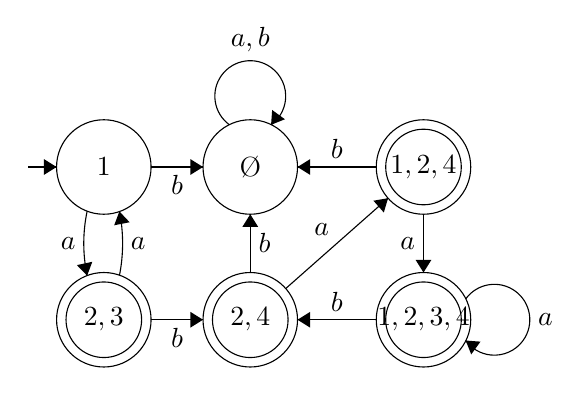
\begin{tikzpicture}[scale=0.2]
\tikzstyle{every node}+=[inner sep=0pt]
\draw [black] (9.2,-10.4) circle (3);
\draw (9.2,-10.4) node {$1$};
\draw [black] (9.2,-20.1) circle (3);
\draw (9.2,-20.1) node {$2,3$};
\draw [black] (9.2,-20.1) circle (2.4);
\draw [black] (18.5,-20.1) circle (3);
\draw (18.5,-20.1) node {$2,4$};
\draw [black] (18.5,-20.1) circle (2.4);
\draw [black] (29.5,-10.4) circle (3);
\draw (29.5,-10.4) node {$1,2,4$};
\draw [black] (29.5,-10.4) circle (2.4);
\draw [black] (29.5,-20.1) circle (3);
\draw (29.5,-20.1) node {$1,2,3,4$};
\draw [black] (29.5,-20.1) circle (2.4);
\draw [black] (18.5,-10.4) circle (3);
\draw (18.5,-10.4) node {$Ø$};
\draw [black] (4.4,-10.4) -- (6.2,-10.4);
\fill [black] (6.2,-10.4) -- (5.4,-9.9) -- (5.4,-10.9);
\draw [black] (12.2,-10.4) -- (15.5,-10.4);
\fill [black] (15.5,-10.4) -- (14.7,-9.9) -- (14.7,-10.9);
\draw (13.85,-10.9) node [below] {$b$};
\draw [black] (8.143,-17.305) arc (-167.99104:-192.00896:9.875);
\fill [black] (8.14,-17.3) -- (8.47,-16.42) -- (7.49,-16.63);
\draw (7.43,-15.25) node [left] {$a$};
\draw [black] (10.194,-13.22) arc (11.19636:-11.19636:10.456);
\fill [black] (10.19,-13.22) -- (9.86,-14.1) -- (10.84,-13.91);
\draw (10.89,-15.25) node [right] {$a$};
\draw [black] (12.2,-20.1) -- (15.5,-20.1);
\fill [black] (15.5,-20.1) -- (14.7,-19.6) -- (14.7,-20.6);
\draw (13.85,-20.6) node [below] {$b$};
\draw [black] (20.75,-18.12) -- (27.25,-12.38);
\fill [black] (27.25,-12.38) -- (26.32,-12.54) -- (26.98,-13.29);
\draw (23.04,-14.76) node [above] {$a$};
\draw [black] (18.5,-17.1) -- (18.5,-13.4);
\fill [black] (18.5,-13.4) -- (18,-14.2) -- (19,-14.2);
\draw (19,-15.25) node [right] {$b$};
\draw [black] (29.5,-13.4) -- (29.5,-17.1);
\fill [black] (29.5,-17.1) -- (30,-16.3) -- (29,-16.3);
\draw (29,-15.25) node [left] {$a$};
\draw [black] (26.5,-10.4) -- (21.5,-10.4);
\fill [black] (21.5,-10.4) -- (22.3,-10.9) -- (22.3,-9.9);
\draw (24,-9.9) node [above] {$b$};
\draw [black] (26.5,-20.1) -- (21.5,-20.1);
\fill [black] (21.5,-20.1) -- (22.3,-20.6) -- (22.3,-19.6);
\draw (24,-19.6) node [above] {$b$};
\draw [black] (32.18,-18.777) arc (144:-144:2.25);
\draw (36.75,-20.1) node [right] {$a$};
\fill [black] (32.18,-21.42) -- (32.53,-22.3) -- (33.12,-21.49);
\draw [black] (17.177,-7.72) arc (234:-54:2.25);
\draw (18.5,-3.15) node [above] {$a,b$};
\fill [black] (19.82,-7.72) -- (20.7,-7.37) -- (19.89,-6.78);
\end{tikzpicture}
\end{center}


\end{document}
